
\section{Experimental Results}
We have written some scripts for some basic graph plotting and some analysis.\\
Below is one of the experimental result.\\
\begin{figure}[!ht]
	\centering
	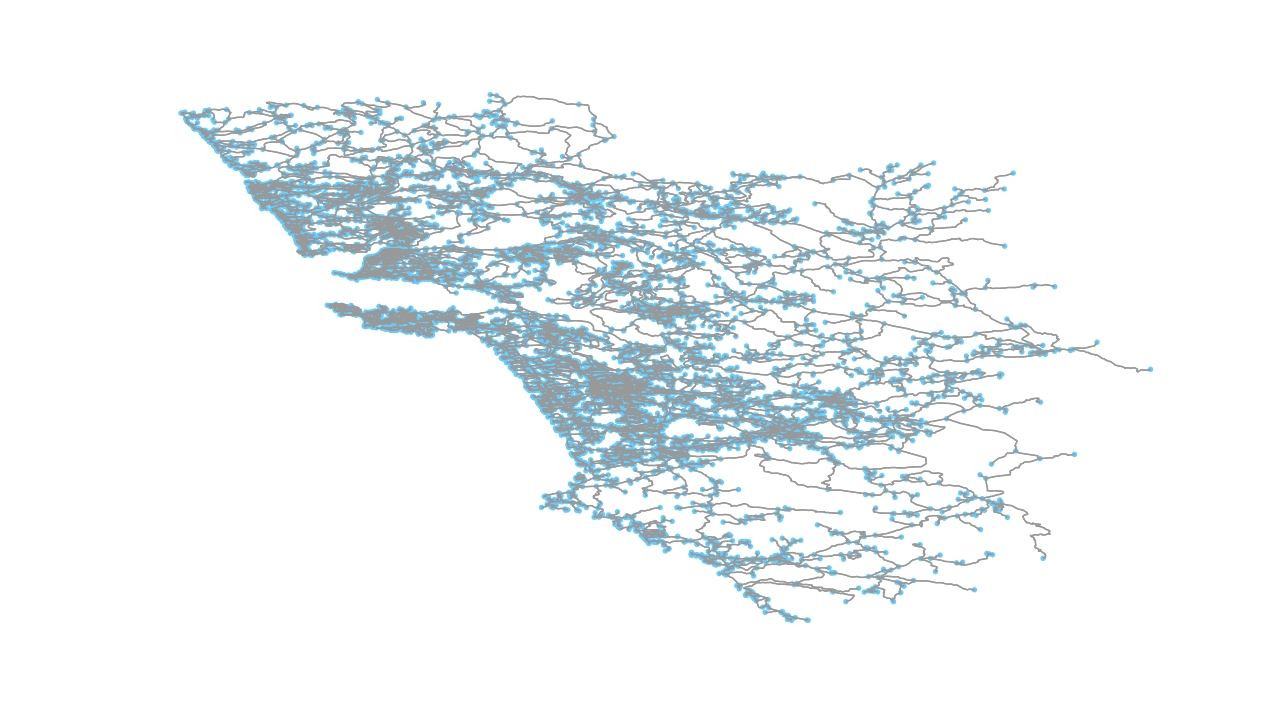
\includegraphics[width=0.7\textwidth]{input/images/plot1.jpg}              
	\caption{Goa Road Network Plotted}
	\hspace{-1.5em}
\end{figure}\\
You may refer to my blogs also for detailed information.\\
Here is the url: \\
http://geoffboeing.com/ \\\\
Road network of Punjab looks like this:
\begin{figure}[!ht]
	\centering
	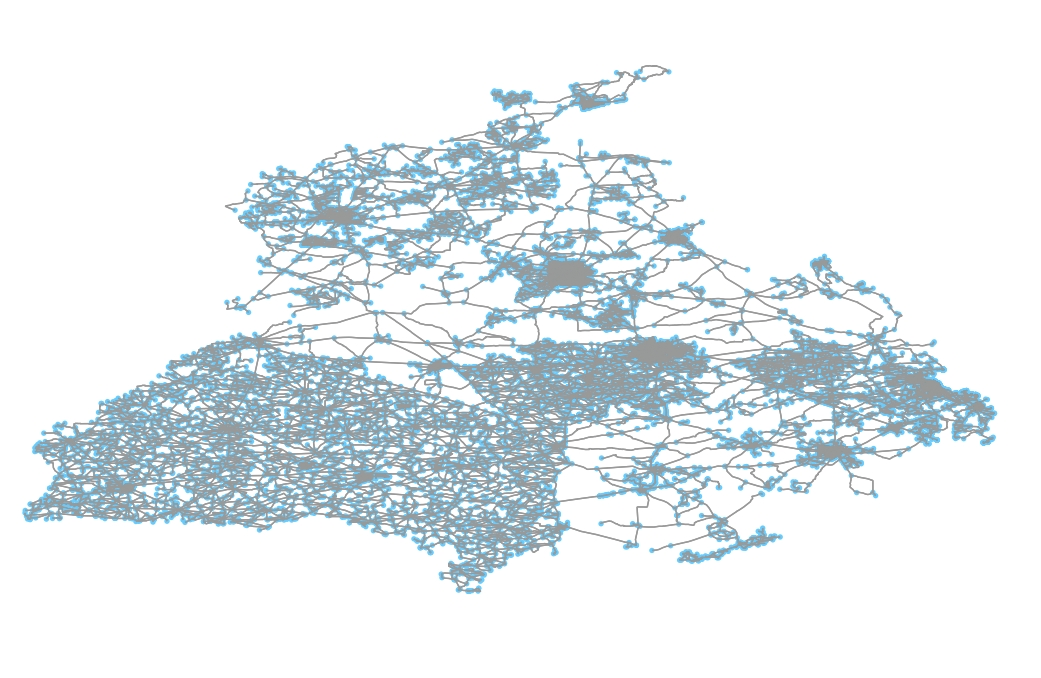
\includegraphics[width=0.7\textwidth]{input/images/p.jpg}                
	\caption{Punjab road network}
	\hspace{-1.5em}
\end{figure}\\\\
\subsubsection{Create Road Networks}
Script to create road networks

\begin{description}
	
	\item [\ import osmnx as ox]
	\item [\ T ="#Place osm tag here"]
	\item [\ ox.plot\_graph(ox.graph\_from\_place(T))]
	
\end{description}

\subsubsection{Create Road Networks}
Script result for finding pagerank using NetworkX:

\begin{figure}[!ht]
	\centering
	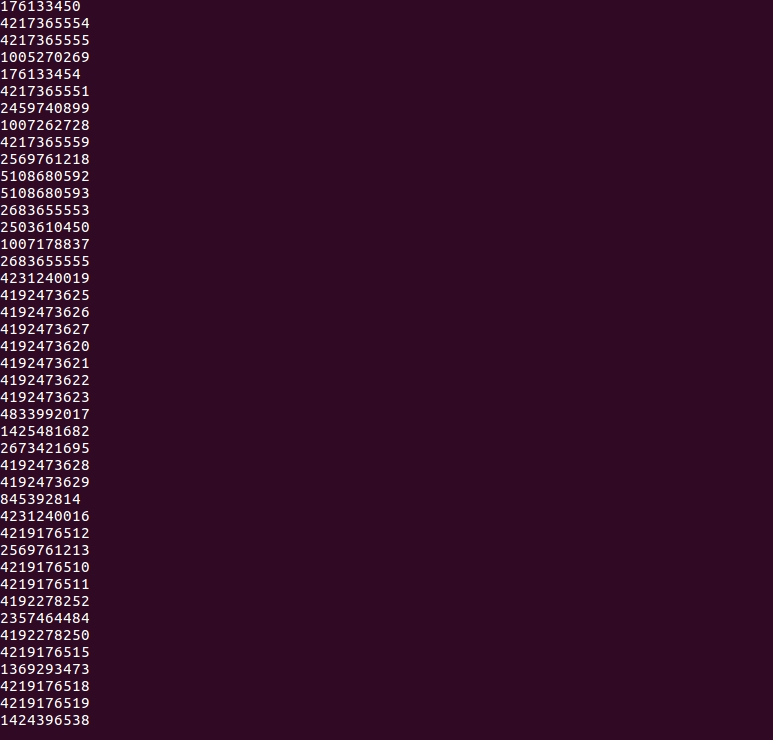
\includegraphics[scale=0.5]{input/images/pg.jpg}              
	\caption{Pagerank using NetworkX}
	\hspace{-1.5em}
\end{figure}\\

\subsubsection{Create Road Networks}
Script result for finding pagerank using GraphFrames:

\begin{figure}[!ht]
	\centering
	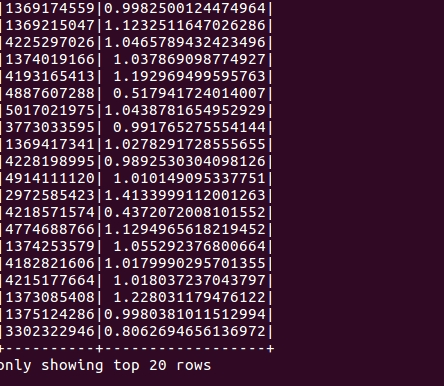
\includegraphics[scale=0.5]{input/images/pggf.jpg}              
	\caption{Pagerank using GraphFrames}
\end{figure}\\
 
\section{Conclusions}
We concluded some information using processing times and other analysis as follows:  
\subsection{When to use NetworkX}
\begin{itemize}
	\item Unlike many other tools, it is designed to handle data on a scale relevant to
	modern problems.
	\item Most of the core algorithms rely on extremely fast legacy code
	\item Highly flexible graph implementations (a graph/node can be anything!)
	\item Extensive set of native readable and writable formats
	\item Takes advantage of Python’s ability to pull data from the Internet or databases
\end{itemize}
\subsection{When not to use NetworkX}
\begin{itemize}
	\item Large-scale problems that require faster approaches (i.e. massive networks
	with 100M/1B edges)
	\item Better use of memory/threads than Python (large objects, parallel computation)
\end{itemize}


\subsection{Isochrone Maps with OSMnx + Python}
How far can you travel on foot in 15 minutes? Urban planners use isochrone maps to show spatial horizons (i.e., isolines) that are equal in time. Isochrones depict areas according to how long it takes to arrive there from some point. These visualizations are particularly useful in transportation planning as they reveal what places are accessible within a set of time horizons.

We can create isochrone maps for anywhere in the world automatically with Python and its OSMnx package:
 
 
You can create your own travel time maps for any city in the world by following this example in the new OSMnx examples GitHub repo. OSMnx is a Python package for easily downloading, analyzing, and visualizing OpenStreetMap street networks anywhere in the world. Installation instructions and demonstrations are on Geoffboing's GitHub.\\
\begin{figure}
	\centering
	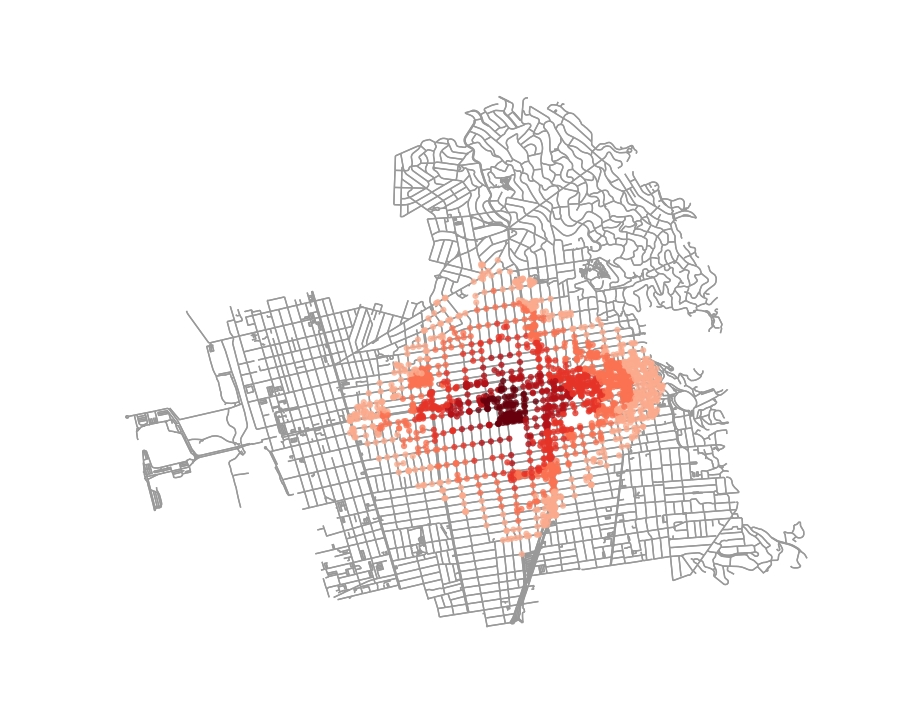
\includegraphics[scale=0.5]{input/images/plot2.jpg}              
	\caption{This travel time map shows how far we can walk in 5, 10, 15, 20, and 25 minutes from an origin point in downtown Berkeley, given an average walking speed of 4.5 km/hour (about 2.8 miles/hour). We can also visualize this by which points along the network we can reach within 5, 10, 15, 20, and 25 minutes}
\end{figure}\\
\subsubsection{Code for fig 5.5:}
\begin{verbatim}
import osmnx as ox, networkx as nx, geopandas as gpd, matplotlib.pyplot as plt
from shapely.geometry import Point
from descartes import PolygonPatch
ox.config(log_console=True, use_cache=True)
# configure the place, network type, trip times, and travel speed
place = 'Berkeley, CA, USA'
network_type = 'walk'
trip_times = [5, 10, 15, 20, 25] #in minutes
travel_speed = 4.5 #walking speed in km/hour# download the street network
G = ox.graph_from_place(place, network_type=network_type)
# find the centermost node and then project the graph to UTM
gdf_nodes = ox.graph_to_gdfs(G, edges=False)
x, y = gdf_nodes['geometry'].unary_union.centroid.xy
center_node = ox.get_nearest_node(G, (y[0], x[0]))
G = ox.project_graph(G)
# add an edge attribute for time in minutes required to traverse each edge
meters_per_minute = travel_speed * 1000 / 60 #km per hour to m per minute
for u, v, k, data in G.edges(data=True, keys=True):
	data['time'] = data['length'] / meters_per_minute
	# get one color for each isochrone
	iso_colors = ox.get_colors(n=len(trip_times), cmap='Reds', start=0.3, return_hex=True)
# color the nodes according to isochrone then plot the street network
node_colors = {}
	for trip_time, color in zip(sorted(trip_times, reverse=True), iso_colors):
	subgraph = nx.ego_graph(G, center_node, radius=trip_time, distance='time')
	for node in subgraph.nodes():
	node_colors[node] = color
	nc = [node_colors[node] if node in node_colors else 'none' for node in G.nodes()]
fig, ax = ox.plot_graph(G, fig_height=8, node_color=nc, node_size=20, node_alpha=0.8, node_zorder=2)

\end{verbatim}
\subsubsection{Code for in fig 5.6}
\begin{figure}
	\centering
	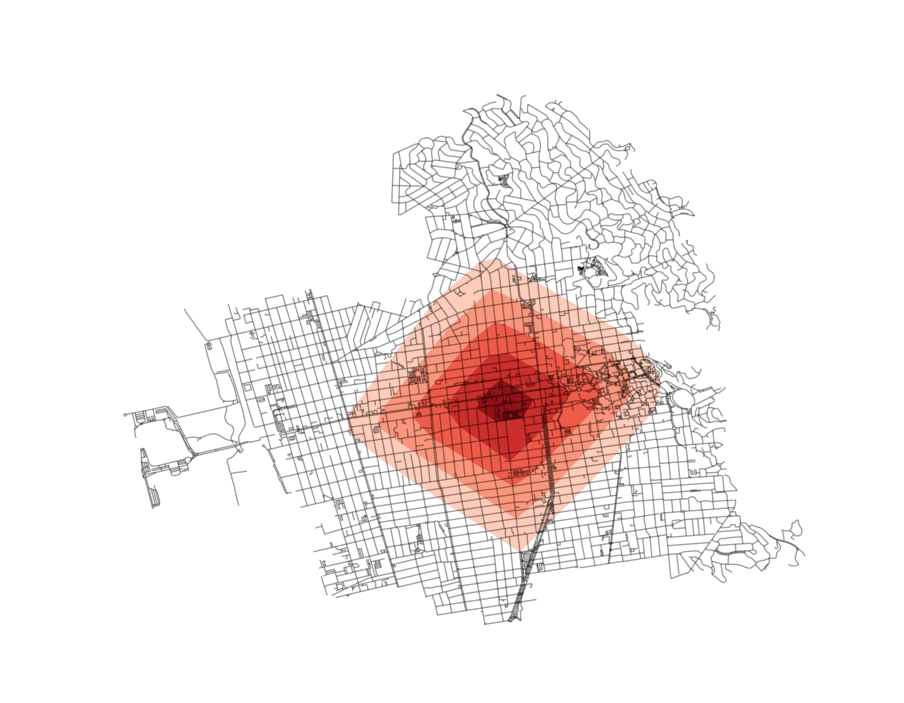
\includegraphics[scale=0.5]{input/images/plot3.jpg}              
	\caption{This travel time map shows how far we can walk in 5, 10, 15, 20, and 25 minutes from an origin point in downtown Berkeley, given an average walking speed of 4.5 km/hour (about 2.8 miles/hour). We can also visualize this by which points along the network we can reach within 5, 10, 15, 20, and 25 minutes}
\end{figure}\\
\begin{verbatim}
import osmnx as ox, networkx as nx, geopandas as gpd, matplotlib.pyplot as plt
from shapely.geometry import Point
from descartes import PolygonPatch
ox.config(log_console=True, use_cache=True)
# configure the place, network type, trip times, and travel speed
place = 'Berkeley, CA, USA'
network_type = 'walk'
trip_times = [5, 10, 15, 20, 25] #in minutes
travel_speed = 4.5 #walking speed in km/hour# download the street network
G = ox.graph_from_place(place, network_type=network_type)
# find the centermost node and then project the graph to UTM
gdf_nodes = ox.graph_to_gdfs(G, edges=False)
x, y = gdf_nodes['geometry'].unary_union.centroid.xy
center_node = ox.get_nearest_node(G, (y[0], x[0]))
G = ox.project_graph(G)
# add an edge attribute for time in minutes required to traverse each edge
meters_per_minute = travel_speed * 1000 / 60 #km per hour to m per minute
for u, v, k, data in G.edges(data=True, keys=True):
	data['time'] = data['length'] / meters_per_minute
	# get one color for each isochrone
	iso_colors = ox.get_colors(n=len(trip_times), cmap='Reds', start=0.3, return_hex=True)
# color the nodes according to isochrone then plot the street network
# make the isochrone polygons
isochrone_polys = []
for trip_time in sorted(trip_times, reverse=True):
	subgraph = nx.ego_graph(G, center_node, radius=trip_time, distance='time')
	node_points = [Point((data['x'], data['y'])) for node, data in subgraph.nodes(data=True)]
	bounding_poly = gpd.GeoSeries(node_points).unary_union.convex_hull
	isochrone_polys.append(bounding_poly)
# plot the network then add isochrones as colored descartes polygon patches
fig, ax = ox.plot_graph(G, fig_height=8, show=False, close=False, edge_color='k', edge_alpha=0.2, node_color='none')
for polygon, fc in zip(isochrone_polys, iso_colors):
	patch = PolygonPatch(polygon, fc=fc, ec='none', alpha=0.6, zorder=-1)
	ax.add_patch(patch)
plt.show()

\end{verbatim}

